\documentclass{article}
\usepackage[utf8]{inputenc}
\usepackage{caption}
\usepackage{amsmath}
\usepackage{amssymb}
\usepackage{mathtools}
\usepackage{multicol}
\usepackage{graphicx}
\usepackage{wrapfig}
\usepackage{float}
\usepackage[makeroom]{cancel}
\usepackage{mhchem}
\usepackage{pst-plot}

\graphicspath{ {../images/} }

\renewcommand{\familydefault}{\sfdefault}
\renewcommand{\baselinestretch}{1.5} % line spacing
\newcommand{\fline}{\par\noindent\rule{\textwidth}{0.1pt}} % horizontal line (wide)

\title{Topic 4 Acids \& Bases\\4.3 - Lewis Acids / Bases}
\author{Peter Zhang}

\begin{document}

\maketitle
\tableofcontents
\newpage

% lesson 
\section{Lewis Acids / Bases}
Lewis structures help fortify the \textbf{Bronsted-Lowry THEORY}. \\For Bases:
\begin{enumerate}
\item Lone pair of electrons (THIS MUST EXIST otherwise its not even a possible option)
\item referred to as the \textbf{nucleophiles} -- electron rich species
\item $\therefore $ Donates a lone pair of electrons
\end{enumerate}
For Acids:
\begin{enumerate}
\item Known as \textbf{electrophiles}
\item electron deficient species
\item $\therefore $ Accepts a lone pair
\end{enumerate}
Basically, bases must contain a lone pair that can be shared. Acids receive lone pairs. If coordinate covalent bonds form, then we have some form of lewis acid or base. 

$$\ce{BF3 + NH3 -> BF3NH3}$$
\begin{figure}[H]
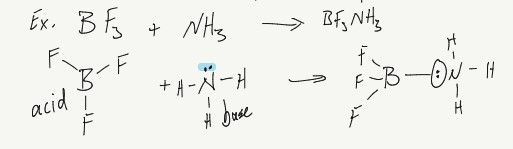
\includegraphics[width=\textwidth]{4.3fig1.jpg}
\captionof{figure}{Reaction between BF3 and NH3}
\end{figure}

The reason why this reaction happens because basically all molecules/elements want a full octet.

$$\ce{MgCl2 + H2O -> Hg(OH)2 + HCl}$$
\begin{figure}[H]
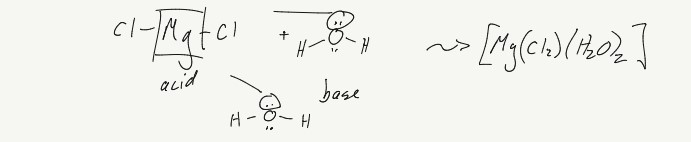
\includegraphics[width=\textwidth]{4.3fig2.jpg}
\captionof{figure}{Reaction between Transition Metal acting as Lewis acid}
\end{figure}
This is what would happen normally. But now that we have lewis acids and bases: Mg has non-full octet. Therefore there is potential for \ce{MgCl2} to act as the acid and \ce{H2O} to act as the base, creating a complex ion \ce{Mg(Cl2)(H2O)2}. Ligand rules and octet rules (H2O is considered a single ligand / single lone electron pair even though it has 2 lone pairs).



%---- page break -----%

Transitional metals capable of d-orbital splitting can also act as Lewis acids with the ligand as a lewis base. 
$$\ce{Cu2+ + 6H2O \rightleftharpoons [Cu(H2O)6]2+}$$

My reaction is very cool



\subsection{Notes about Lewis}
idk this place is empty














\end{document}